% !TEX root = ../../thesis.tex

\chapter{Motivations and Methodology}


\section{TODO}

Majeurs:
2) cependant un points majeur est à argumenter et creuser beaucoup plus en profondeur: le côte open-source. Pour l’instant, le texte fait comme si c’était une évidence que
   i) tout le monde connait les tenants et les aboutissants de l’open-source (il faut les expliquer)
  ii) que c’est intéressant que la méthodologie produise des outils open-source et les diffuse
  ==> ce n’est pas du tout évident et ça doit être argumenté (si c’était évident, pourquoi 99 pourcent des autres travaux en robotique sont pas open source ?)
  ==> Tu dois discuter des avantages, mais aussi des difficultés potentielles qu’implique un projet open-source
 Tu peux te baser sur l’analyse de l’impact du côté open-source dans d’autres projets, e.g. ICub/Darwin, Arduino, etc, et en particulier dans la section 1.3.5 qui doit être beaucoup plus détaillée

Ponctuels:


p. 2: “while acting robustly in the real world?” —> phrase pas claire, on ne voit pas trop ce que tu veux dire
p. 2: “how can we make this work … community” —> 1) anglais par correct; 2) explique en quoi c’est un “epistemological problem”; 3) explique en quoi c’est un problème important

1.2.2: “has never been transferred to another lab” —> explique en quoi c’est un problème (ça n’embête presque personne en robotique, donc il faut faire une discussion ici)




\section{Introduction} % (fold)

In chapter REF(related work sur le corps), we discussed the emergence of novel paradigm in the robotics field that appeared in the late 80's. The embodied artificial intelligence rejects the symbolic approach and postulates that it is not possible to have intelligence without an actual robot body associated with its ecological niche~\cite{pfeifer2001understanding}. Following this paradigm, several researchers tried to tackle challenges in which the classical cognitivist approach failed (see REF) e.g. the understanding of natural forms of intelligence that require a direct interaction with the real world.

Thus an interesting evolution of the last decades is the demonstration of the importance of the morphology for sensorimotor control, cognition and development (\cite{kaplan2008corps} \cite{REF} \cite{REF}). Exploring the interaction between body properties and cognition could lead to both a better understanding of animals’ behaviour (human being in particular) and to build robot more adapted and robust to an open environment with unpredictable interactions. In particular we can highlight the acquisition of sensorimotor tasks and the exploration of adapted bodies for natural physical and social interactions with humans.

In this context, we should not only take care of the robot body design but \textbf{introduce the morphology as an experimental variable and conduct experiments in the real world}. As Rodney Brooks said \emph{the world is its own best model}~\cite{brooks1991intelligence} and simulators cannot handle the complexity of the real physic with multi-point contacts, soft materials and frictions. This is especially the case of complex dynamic tasks such as physical interaction or legged locomotion.


Following the definition of the robotic morphology given by C.Paul:
\begin{quotation}
    The morphology of a robot thus refers to the physical structure and form of a robot. Specifically, the focus is on characteristics such as link sizes, number of links, joint characteristics, mass distribution, actuator characteristics, material properties, sensor characteristics and sensor placements. In short, any characteristic which defines the physical structure of the robot is included in the term morphology.
    \signed{Chandana Paul~\cite{paul2006morphological}}
\end{quotation}

We need to find framework allowing to easily and quickly tune morphological parameters on actual robot to explore and hopefully find new way to improve robot behaviour acting in the real world. However considering the morphology as an experimental variable raised two major epistemological problems:
\begin{itemize}
    \item \textbf{how can we have an experimental robotic platform allowing both to change easily and quickly its morphology while acting robustly in the real world ? }
    \item \textbf{how can we make this work, mainly hardware, diffusible and reusable in the research community ? }
\end{itemize}

In the next sections of this chapter, we will \textbf{suggest novel approaches and design processes to create and produce robotic platform  allowing a free exploration of their control and morphology through experimentations in the real world while being easily diffusible and reproducible in the research community.}

\section{Challenges} % (fold)

The role of the morphology appears as a fascinating open field of research but until now not as much explored.
We presented in chapter REF, a review of both commercial and laboratory prototypes robot platforms. It appears the current platforms are not suitable to tackle these challenges. Commercial robot do not permit the exploration of the morphology because they are either not open source or the hardware is to complicated/expensive to be modified while lab prototypes are mainly handcrafted and specifically tuned which make them impossible to be reproduced in another lab. These robots are not suitable mainly because of the chosen approach and technologies used to design and produce them.
Indeed, the classic way to design and produce robot is a complicated, time-consuming and expensive process. To be achieved, the current robotic platforms have required dozens of engineers working for years and the raise of important founding for the production.

In this context, creating a platform reproducible everywhere without special tooling or skills, and in which the morphology can be freely explored raises methodological and design process challenges:

\subsection{Make the morphology variable} % (fold)

Current robotic platform, in particular humanoid ones, have mechanical parts either handcrafted or produced with classic machining technique based on milling or casting various metal alloy or plastic.
These techniques require specific upfront tooling which make the production of small batch really expensive. Also, to keep the robot cost rather low, scale effect trough mass production is needed. In this context, current robotic platform cannot have their morphology modified because it would require redoing most of the production process. In addition, the design of such mechanical part is constraints because the manufacturing process implies constraints and the complexity of a part greatly increases its cost. The same issues appear with electronics and the robot sensor space which is, in most cases, frozen. Thus the classic way to design and produce robot is not adapted to the free exploration of the robot morphology, novel design and production paradigm have to be used.

In addition, exploring the role of morphology requires to actually change the morphology. Therefore the access to the whole source files should be free allowing anyone to modify them accordingly to their needs and then produce novel designs.

\subsection{Create reproducible robot prototypes} % (fold)

Several interesting robotic platforms explore key aspects in the robot morphology, we can cite Kenshiro~\cite{REF} which uses complex and bio-inspired artificial muscles actuator network, or semi-passive walkers such as Denise~\cite{REF} demonstrating impressive walking ability with few control and power actuation. Unfortunately, none of these robots can be and has never been transferred to another lab. Indeed their production requires specific tooling and hand tuning only few skilled people have.


\begin{figure}[tb]
    \begin{center}
        \includegraphics[width=0.8\linewidth]{step2_troll.jpg}
    \end{center}
    \caption{Caption here}
    \label{fig:figure1}
\end{figure}

 where there’s unfettered access to knowledge and the components associated (articles, data, software, materials, methods), where work can be built upon without asking permission (setting our eyes on reproducibility), and where our modus operandi is more rooted in open collaboration (and we’re rewarded for such behavior).

However one basis of Science is its universality i.e. the fact something can be

To enhance scientific impact, our work should be reproducible in another lab. This is essential as it permits the validation of scientific results presented in publications, and it enables cumulative science which permits to accelerate the development of new technology. Also we are especially attentive to these criterion:

\begin{description}
    \item[Precision, stationary] Experiments should be repeatable, implying that the robot morphology properties should be stationary. This means the robot performances should not be dependent of the place where it has been built nor people skills.
    \item[Easy and fast to duplicate:] Such a reuse of the robotic platform requires that it is easy and fast to duplicate and does not rely on specific tooling or exotic components.
    \item[Affordable:] To ensure a wide spread, a key aspect is to keep the cost of platform relatively low. More labs can be involved more the scientific impact is.
\end{description}


\subsection{Keep robotic platform simple and easy-to-use} % (fold)
The robotic field is intrinsically multidisciplinary. A robot itself requires technologies coming from mechanics, electronics and computer sciences, but the scientific impact of robotics can be way larger and reach non-engineering fields such as human, social or biological sciences. Thus robotic field is an expert field where nobody can be expert in each required skills.
We have to take into account the fact the end user is certainly expert in one specific field but beginner in the other fields. This mean that in each field, the designed robot has to be simple enough to be understood and used by beginners while having, at the same time, enough potential to not constrain users in their expertise field.


\section{The chosen approach} % (fold)

To address these challenges, we suggest exploring an alternative design methodology which is driven by the desire to:
\begin{itemize}
    \item freely explore morphological properties,
    \item reduce the required amount of time between an idea and its experimentation on an actual robotic platform in the real life,
    \item make our work easily reproducible in any other labs,
    \item keep our work modular and free-to-use following open source principles so it can be reused and extended for other project.
\end{itemize}


\subsection{3D print mechanical parts} % (fold)
We could think of having classical mechanical parts but reconfigurable and adjustable, allowing for example to explore different length of a link or different centre of mass position. However, this limits the morphological exploration to few dimensions with limited range.

As we discussed in chapter REF, since few years, novel techniques, especially 3D printing are revolutionizing the way we can produce objects. 3D printers open new horizons for the production of mechanical part, they are able to produce parts which were either not possible or extremely expensive with classical techniques (see \figurename~\ref{fig:complex_3D_printed_part}) but also completely change paradigm associated with production. Indeed the cost does not change with the quantity or the complexity, meaning designers are free to explore the shape they want with almost no constraints.

\begin{figure}[!h]
\centering
    \subfloat[][]{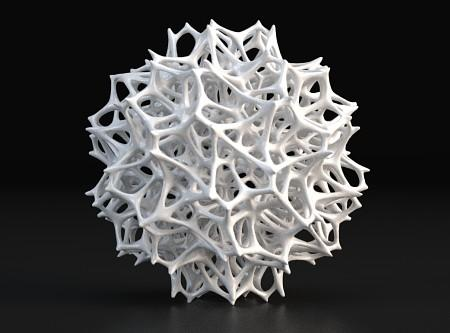
\includegraphics[width=0.4\linewidth]{complex_3Dprinted_part.jpeg}}
    \hfil
    \subfloat[][3D printed metal heat exchanger]{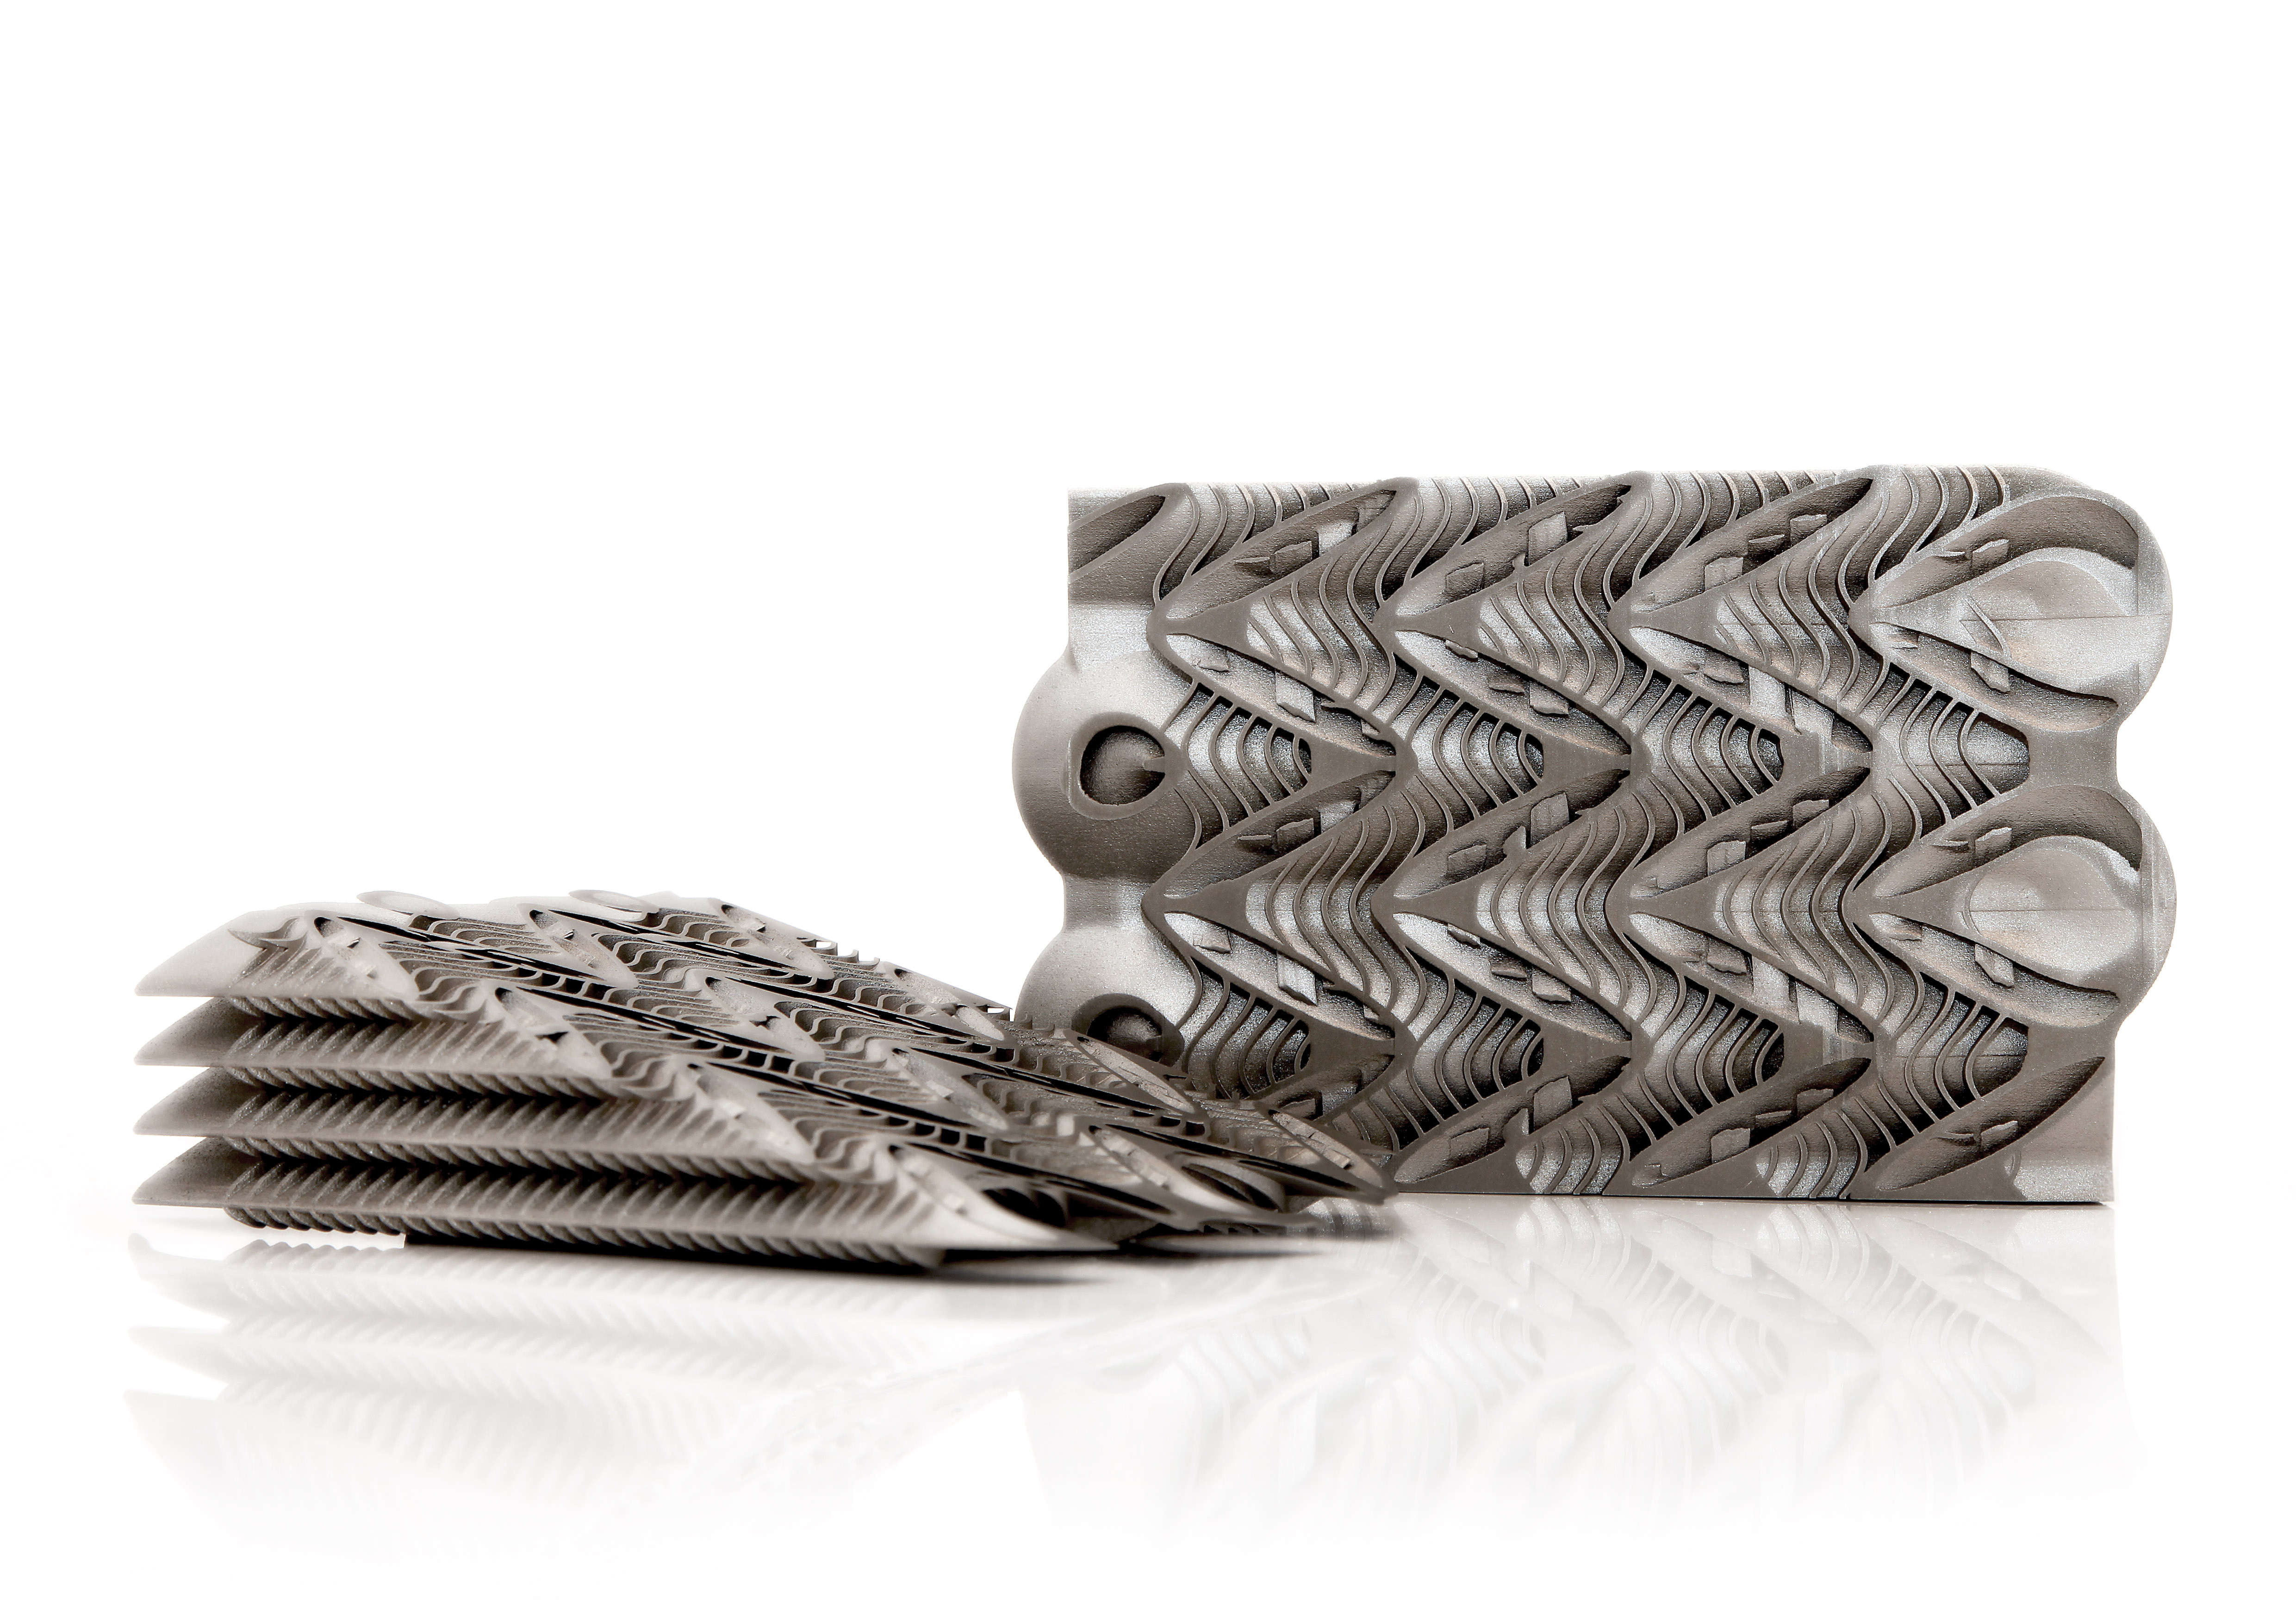
\includegraphics[width=0.55\linewidth]{complex_heat_exchanger.jpg}}
    \caption{}
    \label{fig:complex_3D_printed_part}
\end{figure}


Also, these novel techniques come with the open hardware and makers revolution which brought low cost 3D printer to home. The production of mechanical part can be now done in few hours directly on site with limited human handling.

\begin{figure}[!h]
    \begin{center}
        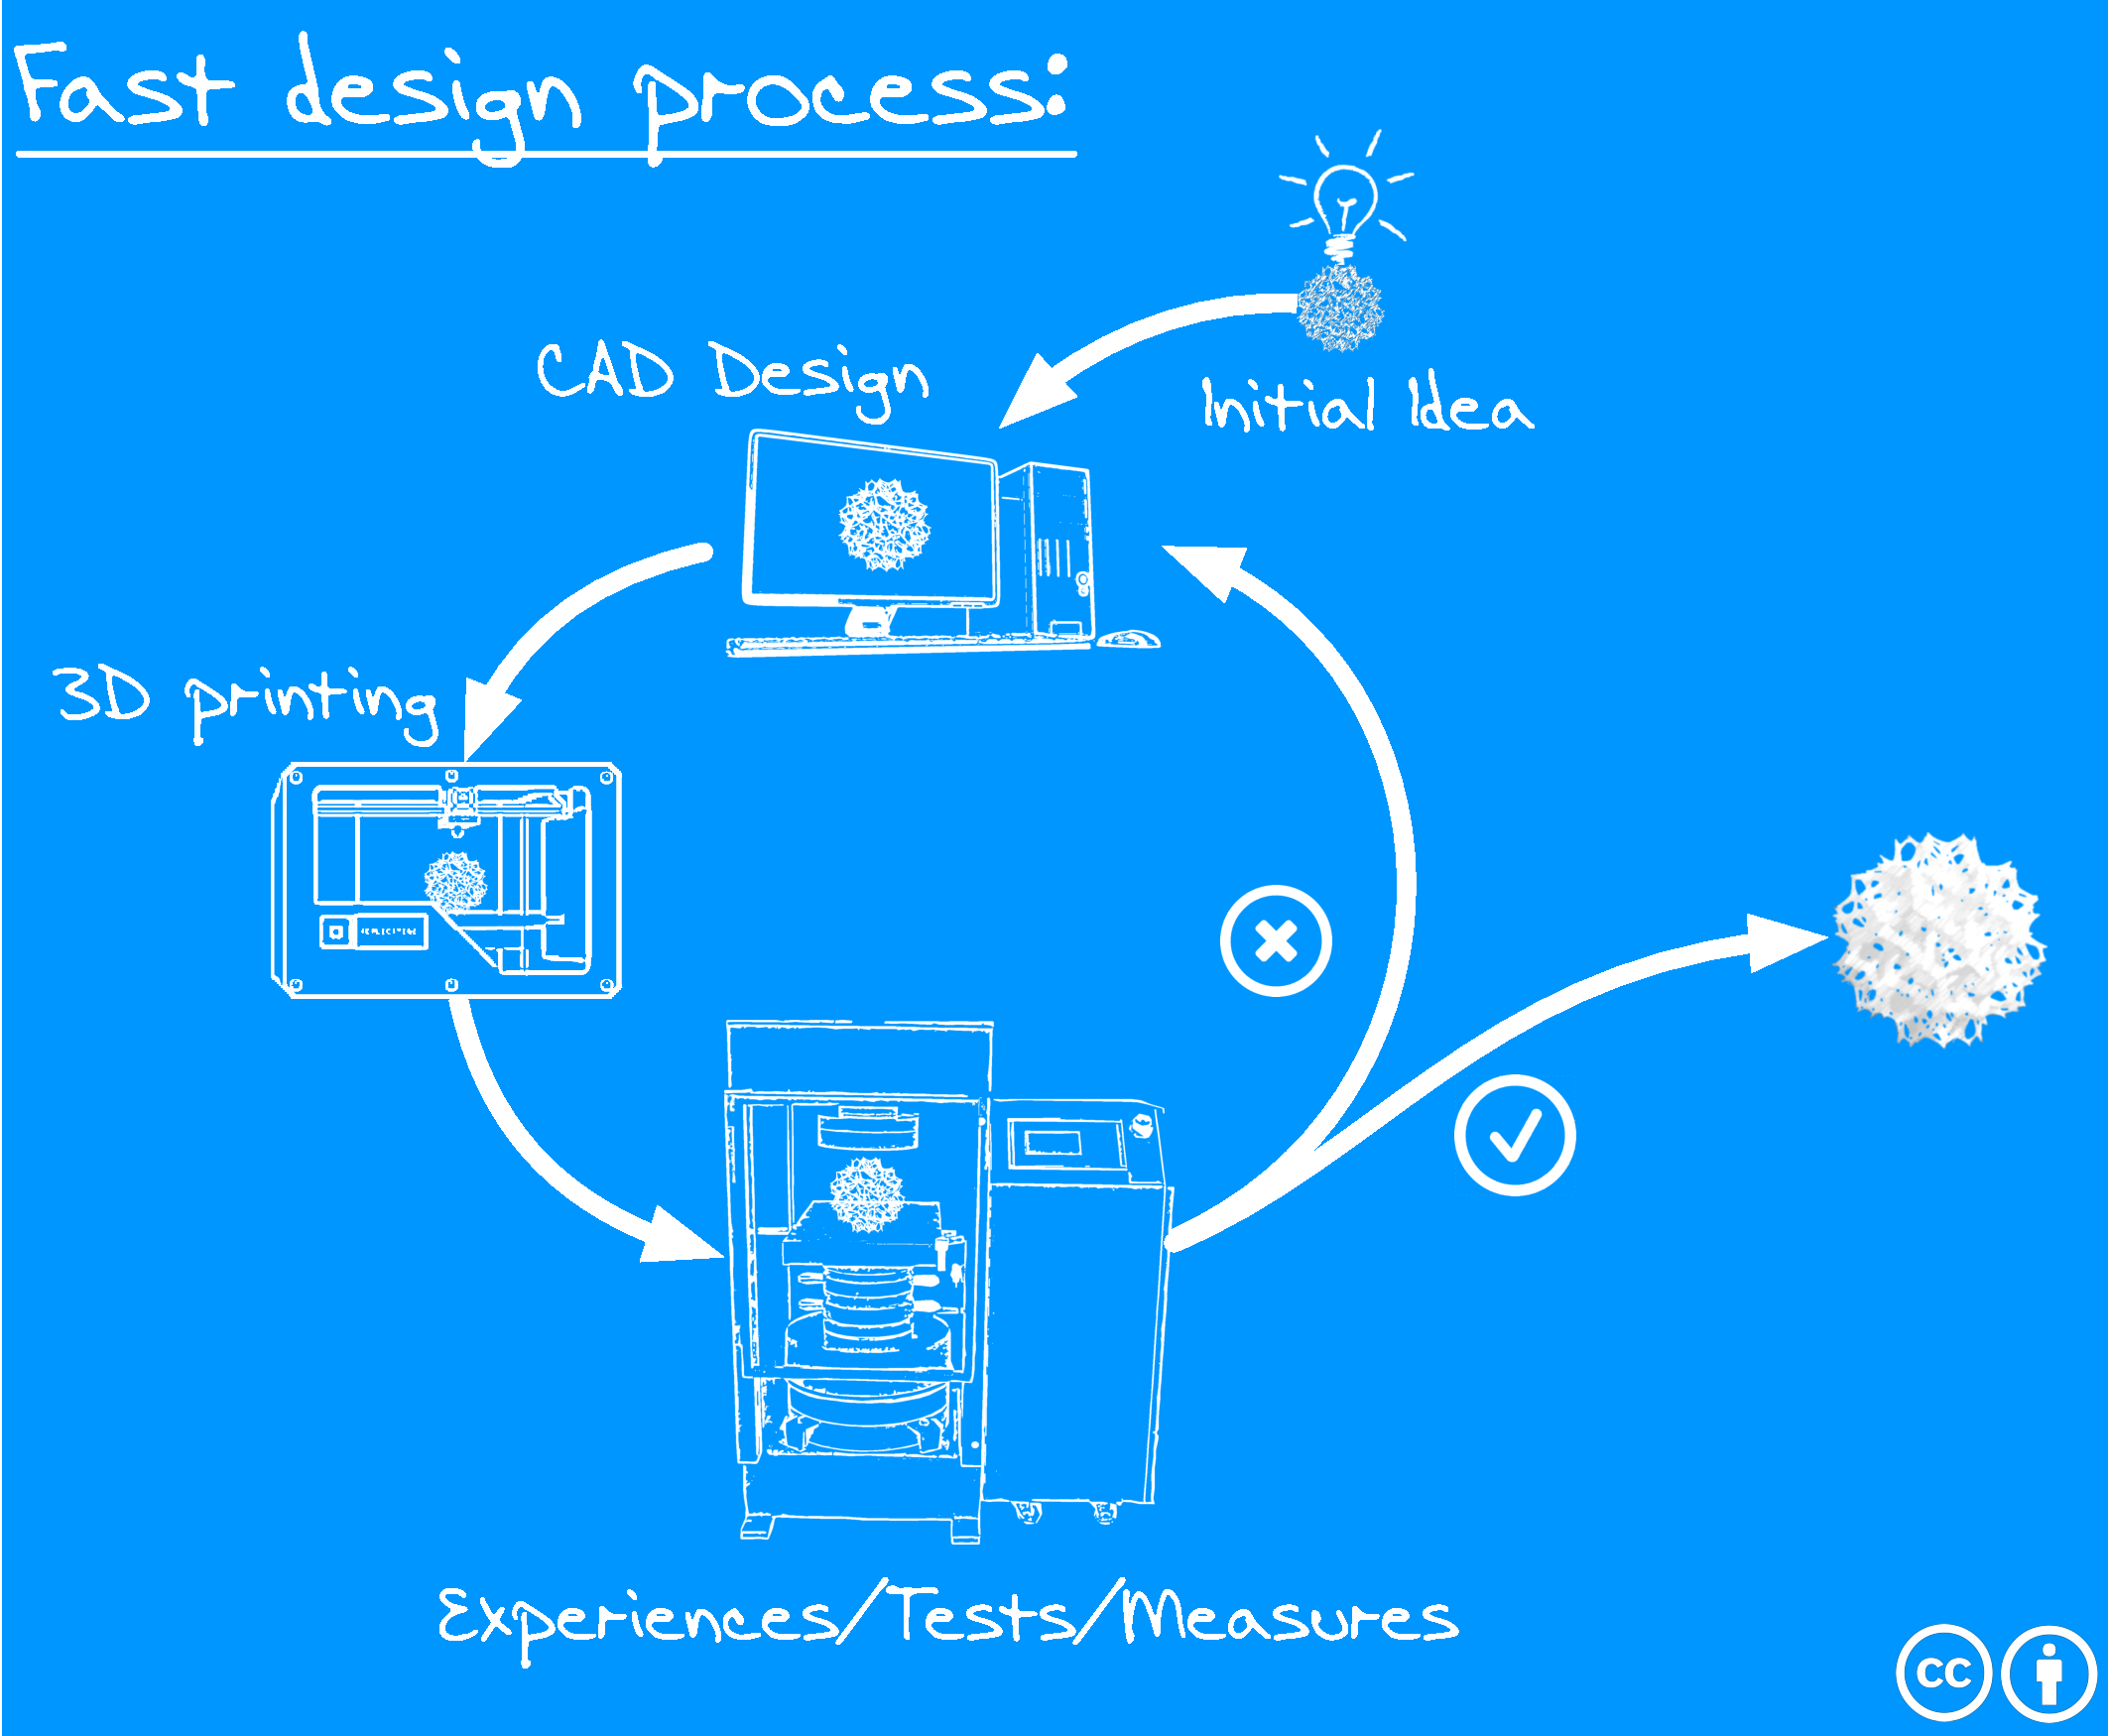
\includegraphics[width=\linewidth]{conception_iterative.pdf}
    \end{center}
    \caption{Fast conception loop}
    \label{fig:conception_loop}
\end{figure}

The 3D printers have several key abilities:
\begin{description}
    \item[Worldwide:] 3D printed part can be obtained everywhere. Either by personal printing or by ordering part other web service such as i.materialise, shapeways or sclupteo.
    \item[Low cost:] The cost to produce 3D parts is rather low cost, it can be from dozens of cents if produced on personal printer to dozens of euros if ordered though web service.
    \item[Fast:] In a couple of hours a whole part can be created from scratch. Using web service, it is needed to add the queue and shipping delay which increase the production time to several days.
    \item[Skill-free:] While the production process is fully numerical, few or no special skills are required.
    \item[Multi-material, precise and robust:] the current 3D printers can create precise (up to 0.1mm) part in different material such as nylon, PLA, ABS or even titanium and flexible material. The obtained parts are robust and can be used as final parts for several years.
    \item[Reduce the number of part:] 3D printing permits to print complex part and even assembled part as complex as bearing or gearbox. This means we can replace multiple parts which have to be assembled into one ready-to-use.
\end{description}

These properties of the 3D printing process enable for the first to really explore morphological variant of mechanical parts. Indeed, it is now fast and low cost to create alternative design. Associated with modular architecture, we can easily and quickly change robot parts and conduct experiment. Also this process is compatible with the diffusion goals while it is simple and accessible anywhere with Internet connection and a mailing address.


\subsection{Electronic architecture based on Arduino} % (fold)

Thanks to 3D printing, exploring morphological variant of mechanical part is now way easier than ever before but unfortunately the printing of electronic components and board is not yet available. However, exploring the role of morphology does not only concern the mechanical properties but also the sensors apparatus i.e. \textbf{which sensor is used and where is it placed on the body}. The Swiss bot (see REF) is a great example of the impact of the sensors position on the robot behaviour.

To permit the exploration of sensor-system variants, we suggest basing the electronic architecture on Arduino. Arduino is an open-source electronics platform based on easy-to-use hardware and software. It's intended for anyone making interactive projects. Arduino board can sense the environment by receiving inputs from a wide variety of sensors, and affects its surroundings by controlling lights, motors, and other actuators. It is not needed to have low-level en embedded programing skills while Arduino boards can be programmed using Arduino programming language\footnote{\url{http://arduino.cc/en/Main/Software}} which abstracts all the complexity.

\begin{figure}[]
    \begin{center}
        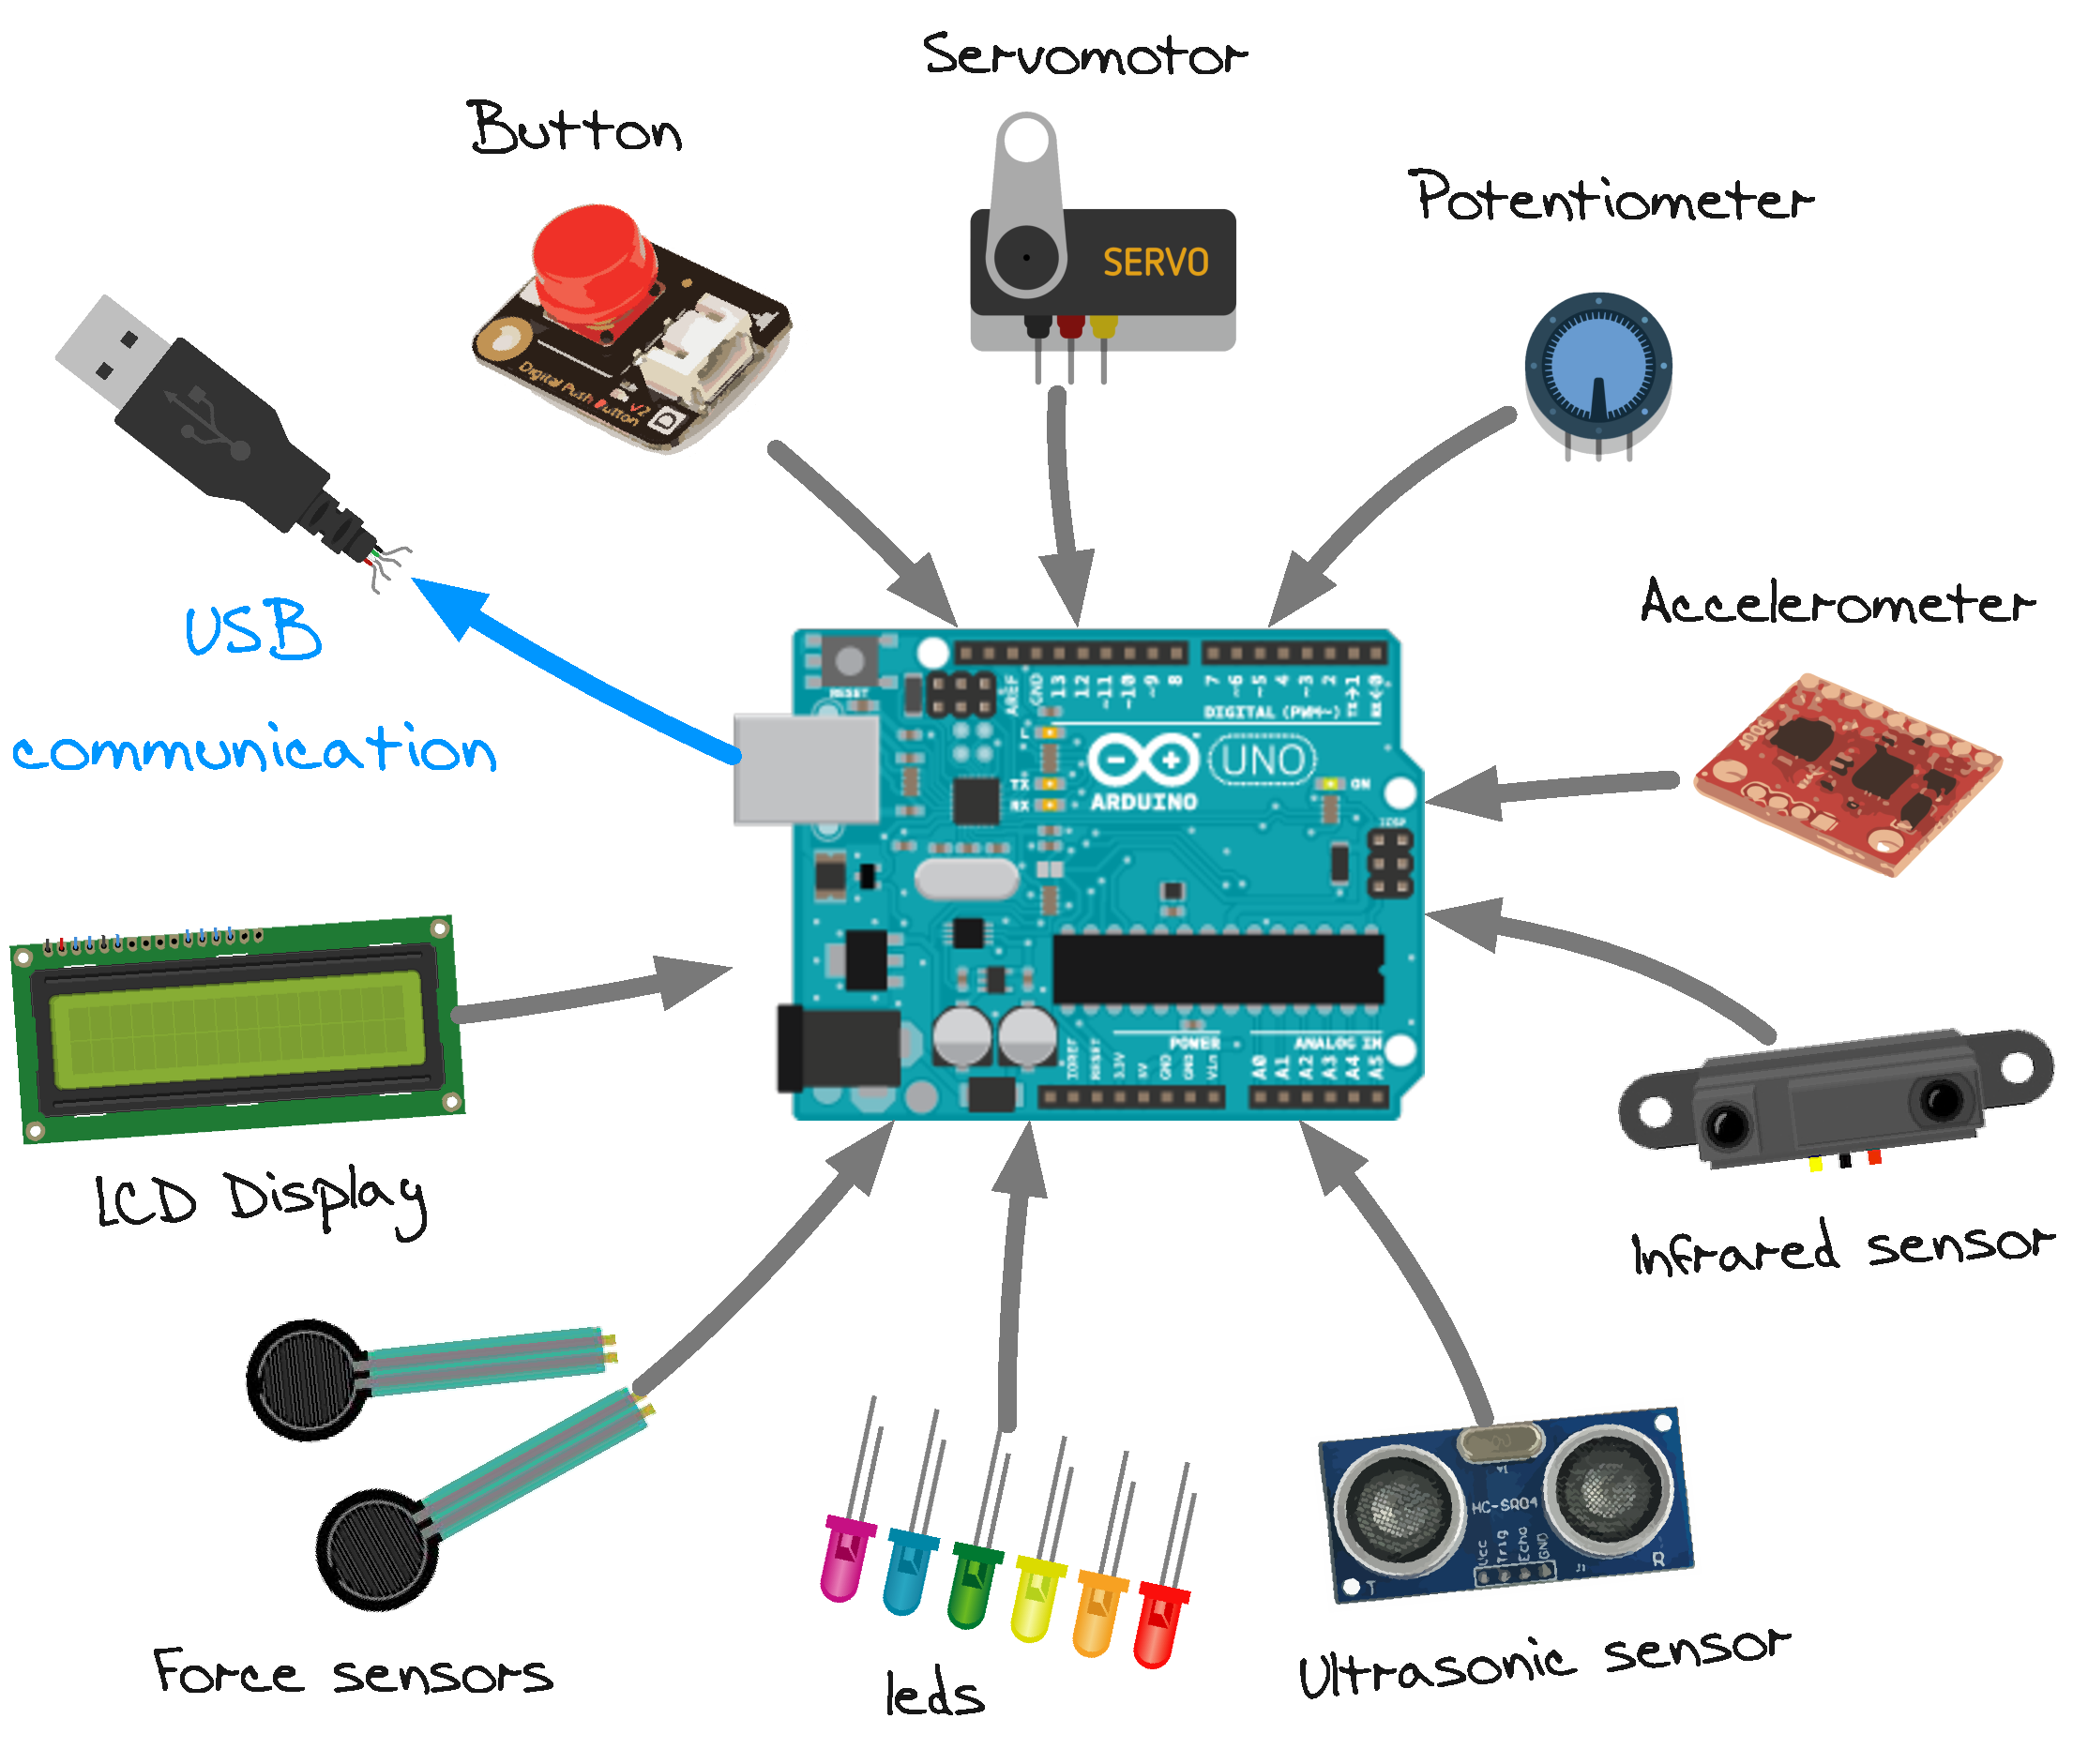
\includegraphics[width=\linewidth]{arduino_electronique.pdf}
    \end{center}
    \caption{The use of Arduino as electronic architecture permit to easily add and/or change sensors while keeping the same electronic board. In addition, it permits to add expressive components such as leds, LCD or sound system allowing user to easily explore human-robot interaction.}
    \label{fig:arduino_modular_electronic}
\end{figure}


The Arduino community is very active and expanding, more and more sensors are designed to be directly plugged on Arduino boards. Thus using Arduino adds modularity to robot electronic architecture, allowing reconfiguring the sensors space by easily adding new one (see \figurename~\ref{fig:arduino_modular_electronic}).




\subsection{All-in-one actuators} % (fold)

As we explained shortly in REF, several techniques are available to make robot move from classic and cheap servomotors to highly powerful and dynamic hydraulic actuators powering the Atlas humanoid robot.
While some actuator technologies such as Series Elastic Actuator (SEA), cable-driven or artificial muscles are really promising to create more robust and efficient robots, they are still working-in-progress solutions and require advanced skills both to be assembled and used.

These technologies are not yet compatible with the creation of diffusible and reproducible robotic platforms in a multidisciplinary research community.


\textbf{TODO: Image de systeme mecanique avec cable ou air }

To permit the diffusion, we need off-the-shell and stationary solutions, easy to assemble, easy-to-use and available anywhere. Also, to allow the exploration of the morphology, actuators have to be modular and permit to explore several parameters.

We therefore chose to use Robotis Dynamixel servo-motors\footnote{\url{http://www.robotis.com/xe/dynamixel_en}} for the robot actuation (see \figurename~\ref{fig:dynamixel_models}). Dynamixel motors are easily accessible while they are mass produced and worldwide shipped. Also they are the most common used actuators in the robotic field and plenty of robot are powered by them among them Darwin-OP~\cite{REF}, Myon~\cite{REF} , Acroban~\cite{REF} or Nimbro~\cite{REF}.

The Dynamixel motors are not simple servomotors, they are all-in-one-modules which contain drivers, encoders and communication bus. They are also quite powerful, robust and rather precise. This is done by the combination of Maxon motors, metal gearbox and precise magnetic rotation sensor (resolution: 0.1\textsuperscript{o}). They embed a 32bits micro-controller dedicated to the communication (serial port TTL or RS232), the control of the joint (position, speed or torque) and the measurement of several internal data such as the real position, speed, load or temperature. They also allow tuning the internal PID or limiting the maximal torque. This permits rich behaviours useful both for physical interaction and locomotion.


\begin{figure}[!h]
\centering
    \subfloat[][Robotis Dynamixel AX and MX series]{\label{fig:dynamixel_models}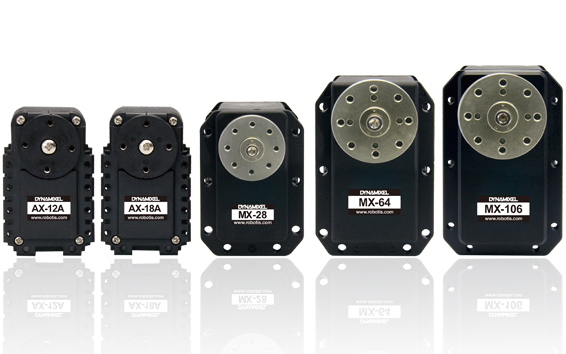
\includegraphics[width=0.48\linewidth]{dynamixel_actuator.jpg}}
    \hfil
    \subfloat[][Power of each Dynamixel model]{\label{fig:dynamixel_powa}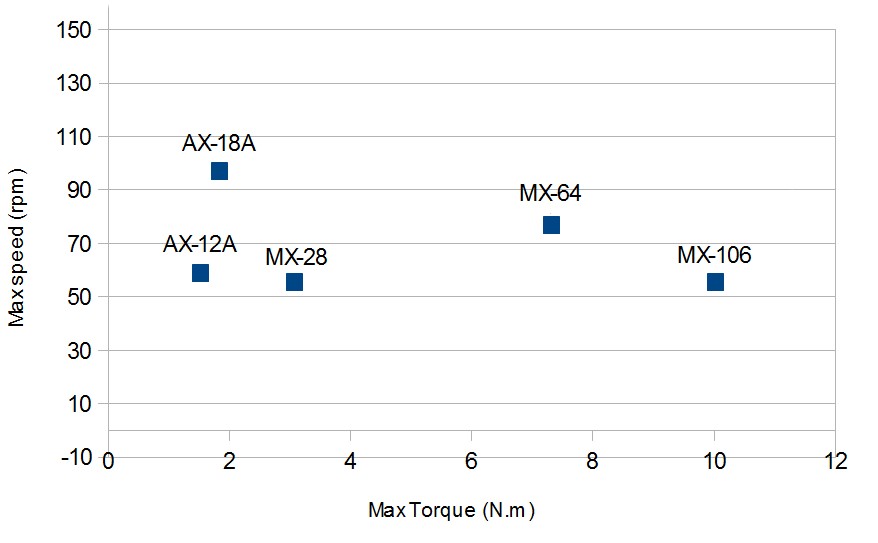
\includegraphics[width=0.48\linewidth]{comparaison-servomoteurs-dynamixel-robotis.png}}\\
    \caption{The Robotis Dynamixel come with different models from low cost ones such as AX-12/18 to the most powerful MX-series with maxon motor and magnetic encoder.}
    \label{fig:dynamixel_serie}
\end{figure}

Different models are available and permit to adjust the actuation to the power required by the joint (see \figurename~\ref{fig:dynamixel_powa}). They are different in size and power but their API remains the same and we can easily switch from one to another without neither changing the code nor the electronic integration. Yet, even if the size change, the foot-print keep the same pattern (see \figurename~\ref{fig:dynamixel_dimension}) which make easy to configure parametric mechanical part, it just takes a couple of minute to transform a part designed to be compatible with Dynamixel MX-28 to one compatible with Dynamixel MX-64.


\begin{figure}[tb]
    \begin{center}
        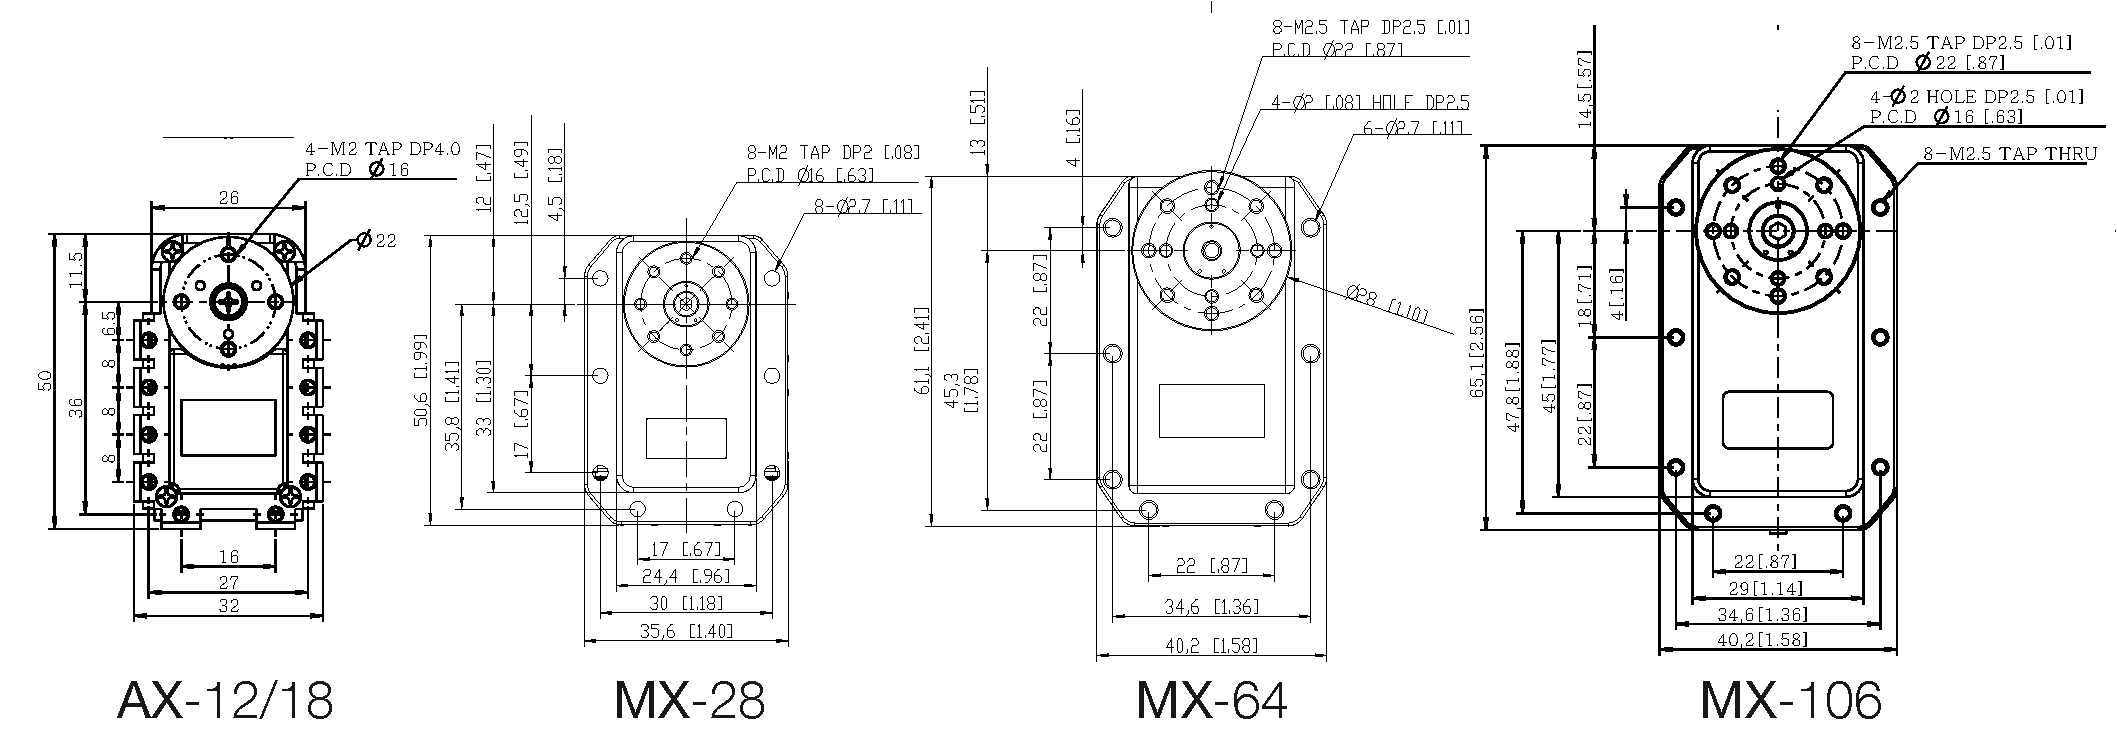
\includegraphics[width=\linewidth]{dynamixel_dimension.pdf}
    \end{center}
    \caption{The footprint of Dynamixel motors keeps the same pattern, just the dimension are increased following the power of the motor. Thus switching from one model to another only requires to change dimension and not the design of a part. With parametric software as Solidworks, it takes a couple of minute to modify a mechanical part to be compatible with another Dynamixel motor.}
    \label{fig:dynamixel_dimension}
\end{figure}


\subsection{Accessible and extensible software} % (fold)

Having variability in software is more classical. Here the choice has been made toward ease-of-use and modularity. We design sensory-motor control API adapted to the hardware variability we have. We choose to use Python as main programming language as it allows fast development, easy deployment on all operating system and quick scripting by non-necessary expert developers. It also offers a large variety of scientific and machine-learning libraries used in robotics (e.g. Numpy, Scipy, Scikit-learn).
This language is rather slow compare to C or Java, but sensorimotor control is done using serial bus communication and as the serial communication is handled through the standard library we can still achieve rather high performance.


\subsection{Open source diffusion} % (fold)

Finally, one of the most important point is the release open source of

Following open source principle, we want to enable open science by sharing all our work


\textbf{TODO Figure ?}

Last but not least, one our main challenge is to enable diffusion and reproduction of robotic platform designed with this approach in the scientific community. While the main aspect of such approach is to create variability, reuse and modification of initial design, it is necessary to not only diffuse our work through scientific publications but also distribute sources in the community. For this purpose we use open source license: GPLv3 for software (Control API) and Creative Commons BY-SA License for Hardware (mechanical parts and electronic boards).

In addition, while our work is intended to be reused by external and hopefully numerous of people, the sources have to be clean, robust and well-documented.


\begin{itemize}
    \item reuse in laboratories
    \item open data
    \item science cumulative
    \item shows the parameter of code
\end{itemize}


\section{Conclusion} % (fold)

In this thesis, we aim to enable both the free exploration of morphological variant on real robotic platform and to permit their diffusion in the research community. To do so, we suggest to explore an alternative design based on 3D printing for mechanical parts, Arduino electronic architecture for sensors, Robotis Dynamixel motor for actuation and Python API for control.

This design process permits to create low cost and highly hackable experimental robotic platform thanks to a fully modular approach.

The tools used take part of the makers revolution and emergence of the "internet of things" sometimes called the novel industrial revolution~\cite{anderson}. Therefore we can rely on the hundreds of Fablab around the world as lever arm to increase the dissemination and replicability of robotic platforms designed with such methods.

Yet the chosen approach raised some limitations. Indeed, while we want to keep our work reproducible, we have to reduce the complexity of the assembly and the use of our robotic platforms. This means we need to spend more time developing and testing our design to make it as easy to use as possible. Also we are limited in the components we can use, they have to be easily accessible i.e. easily available and with quantity toward web stores.


In the next chapter, we will apply this methodology to the design a whole new humanoid robot: Poppy.


